\documentclass[12pt]{article}
\usepackage[UTF8]{ctex}
\usepackage[margin=2cm,a4paper]{geometry}

\usepackage{setspace} %设置行间距

\usepackage{caption}
\usepackage{lipsum}
\usepackage{amsmath}  % 此处引入数学公式的包
\usepackage{graphicx} % 用于插入图片
\counterwithin{figure}{section}
\usepackage{multirow} % Required for multirows,多行表格
\usepackage{subfigure} % 用于两张图片并排排放
\numberwithin{equation}{section} %编号带有章节
\usepackage{listings} % 代码
\usepackage{xcolor} % 高亮
\usepackage{appendix}


\begin{document}
% \maketitle
\begin{titlepage}
\begin{center}
    \begin{figure}
        \centering        
        
\includegraphics[width=0.3\textwidth]{Fig/Harbin_Institute_of_Technology_logo.svg} 
    \end{figure}
    \textbf{\LARGE{\fontfamily{cmr}\selectfont Harbin Institute of Technology}}
\end{center}


\vspace{4em}

    

\begin{center}
    \textbf{\Huge{非线性滤波及信息融合大作业(目标定位)}}
\end{center}

\vspace{8em}

\begin{flushleft}
\begin{spacing}{2}
    \hspace{14em} \textbf{\large{姓名:\underline{\hspace{1.4em}\hspace{2em}}}}\\
    \hspace{14em} \textbf{\large{学号:\underline{\hspace{1em}\hspace{1em}}}}\\
    \hspace{14em} \textbf{\large{学院:\underline{\hspace{1em}\hspace{1.6em}}}}
\end{spacing}
\end{flushleft}


\vspace{8em}
\begin{center}
    \textbf{\large{2023年11月24日}}
\end{center}
\thispagestyle{empty} % 隐藏页码
\end{titlepage}
\newpage

\tableofcontents    % 目录
\thispagestyle{empty} % 隐藏页码
\newpage
\setcounter{page}{1} % 设置本页的页码为1

\section{一阶扩展卡尔曼滤波}
\subsection{一阶扩展卡尔曼滤波原理}
标准卡尔曼滤波方法是建立在线性系统和高斯分布两个假设条件之上的,然
而绝大多数实际系统都存在一定程度的非线性,使得原本符合高斯分布的随机变
量经非线性变换后不再满足高斯特性,导致卡尔曼滤波无法直接应用.

为解决非线性系统的滤波问题,将非线性系统进行线性化是最直接的做法,
从而将非线性滤波问题转化为线性滤波问题.线性化是将非线性函数进行
Taylor 展开或者以多项式的方式进行拟合,然后忽略高阶小项得到偏差线性化
函数的过程,根据所取阶数不同可以获得不同的近似精度,一般以多阶线性化获得较高近似精度的,相应的计算量也会比较大.

EKF是一种比较简单的将非
线性方程进行Taylor一阶展开并忽略高阶项的扩展卡尔曼滤波方法,由于其该
方法只是一阶近似,因此当系统非线性较强时会带来较大的截断误差.但由于
EKF方法的小计算复杂度带来的简便性,在工程中,对于一些非线性并不强的系
统仍被广泛使用.
\subsection{一阶扩展卡尔曼滤波方法}
对于以下非线性系统:
\begin{align}
    x_k = f(x_{k-1}) + w_{k-1}\\
    z_k = h(x_k) + v_k
\end{align}
式中,$f(\cdot)$和$h(\cdot)$为非线性方程;$w_{k-1}$和$v_k$为互不相关的高斯高斯白噪声,
其噪声统计特性为:
\begin{align}
    E[w_k] = 0, ~Cov[w_k,w_j] = Q_k\delta_{k,j}\\
    E[v_k] = 0, ~Cov[v_k,v_j] = R_k\delta_{k,j}
\end{align}
式中,$Q_k$为过程噪声方差矩阵;$R_k$为量测噪声方差阵.

将非线性状态方程$f(\cdot)$在状态估计值$\hat{x}_{k-1}$附近展成一阶Taylor级数,可得
\begin{align}
    f(x_{k-1})\approx f(\hat{x}_{k-1})+\frac{\partial f}{\partial x}\biggl\vert_{\hat{x}_{k-1}}\,(x_{k-1}-\hat{x}_{k-1}) + w_{k-1}
\end{align}
式中,
\begin{align}
    \frac{\partial f}{\partial x}\bigg \vert_{\hat{x}_{k-1}} = 
    \begin{bmatrix}
     \dfrac{\partial f_1(\cdot)}{\partial x_1} & \dfrac{\partial f_1(\cdot)}{\partial x_1} & \cdots & \dfrac{\partial f_1(\cdot)}{\partial x_1}\\
     \dfrac{\partial f_2(\cdot)}{\partial x_2} & \dfrac{\partial f_2(\cdot)}{\partial x_2} & \cdots & \dfrac{\partial f_2(\cdot)}{\partial x_2}\\
     \vdots & \vdots &  & \vdots\\
     \dfrac{\partial f_4(\cdot)}{\partial x_4} & \dfrac{\partial f_4(\cdot)}{\partial x_4} & \cdots & \dfrac{\partial f_4(\cdot)}{\partial x_4}
    \end{bmatrix}
\end{align}

同理,将非线性量测方程$h_k(\cdot)$在状态估计值$\hat{x}_{k|k-1}$附近展开成一阶Taylor级数,可得
\begin{align}
    z_k \approx \left.\hat{h}(\hat{x}_{k}|_{k-1})+\frac{\partial\hat{h}}{\partial x}\right|_{\hat{x}_{k}|k-1} (x_{k}-\hat{x}_{k}|_{k-1})
\end{align}
式中,
\begin{align}
    \frac{\partial h}{\partial x}\bigg \vert_{\hat{x}_{k|k-1}} = 
    \begin{bmatrix}
     \dfrac{\partial h_1(\cdot)}{\partial x_1} & \dfrac{\partial h_1(\cdot)}{\partial x_1} & \cdots & \dfrac{\partial h_1(\cdot)}{\partial x_1}\\
     \dfrac{\partial h_2(\cdot)}{\partial x_2} & \dfrac{\partial h_2(\cdot)}{\partial x_2} & \cdots & \dfrac{\partial h_2(\cdot)}{\partial x_2}\\
     \vdots & \vdots &  & \vdots\\
     \dfrac{\partial h_4(\cdot)}{\partial x_4} & \dfrac{\partial h_4(\cdot)}{\partial x_4} & \cdots & \dfrac{\partial h_4(\cdot)}{\partial x_4}
    \end{bmatrix}
\end{align}
令
\begin{align}
    \left.\begin{array}{l}{{H_{k}=\left.\dfrac{\partial h}{\partial x}\right|_{\hat{x}_{k|k-1}}}}\\ {{\left.\zeta_{k}= h(\hat{x}_{k|k-1})-\dfrac{\partial h}{\partial x}\right|_{\hat{x}_{k|k-1}}\hat{x}_{k|k-1}}}\end{array} \right\}
\end{align}

则非线性量测方程的一阶线性化结果为:
\begin{align}
    z_k = H_k x_k + \zeta_k +v_k
\end{align}

\section{建模过程}
\subsection{问题描述}
假设有三架无人机对移动目标进行协同定位,每架无人机上安装有被动雷达导引头,可提供高低角及方位角两种量测信息.请根据以下仿真条件,完成基于扩展卡尔曼滤波的协同定位滤波器设计及仿真分析.
\subsection{仿真条件}
\begin{enumerate}
    \item 初始时刻,地面系下目标状态位置初值:$p=[x, y, z]=[653.42,567.81,590.61]$ $m$;速度初值:$v=[v_x,v_y,v_z]=[89.93,61.87,84.41]$ $m/s$;加速度初值:$a=[a_x,a_y,a_z]$ $m/s^2$; 目标状态初值的误差:位置误差$\Delta p =[500,500,500]$ ;速度误差$\Delta v = [50, 50, 50]$;加速度$\Delta a = [5,5,5]$ (用于构造误差协方差矩阵初值).
    \item 目标运动模型选用"当前"统计模型,机动系数可选为$\dfrac{1}{60}$;
    \item 导引头测角噪声为零均值高斯噪声,标准差$\sigma = 0.5^{\circ}$;
    \item 导引头测量帧频为$10\mathbf{HZ}$,共$40\mathbf{s}$;
    \item 不考虑无人机姿态变化,并假设无人机本体系与地面系重合.
\end{enumerate}

\subsection{"当前"统计模型}
以地理系为参考坐标系,选取地理系下目标运动的位置$(x,y,z)$,速度$(v_x,v_y,v_z)$,加速度$(a_x,a_y,a_z)$为状态变量,有
\begin{align}
    X = [x,y,z,v_x,v_y,v_z,a_x.a_y,a_z]
\end{align}

根据"当前"统计模型建立的目标运动离散化方程为
\begin{align}
    X_k = \Phi_{k|k-1}X_{k-1} + U_{k-1}\bar{a_k} + w_k
\end{align}
其中,状态转移矩阵分别为
\begin{align}
    \Phi_{k|k-1}=\left[
        \begin{array}{c c c}
        {{I_{3\times3}}}&{{T\cdot I_{3\times3}}}&{{\frac{1}{\alpha^{2}}\left[-1+\alpha\cdot T+e^{-\alpha T}\right]\cdot I_{3\times3}}}\\ {{0_{3\times3}}}&{{I_{3\times3}}}&{{\frac{1}{\alpha}\left[1-e^{-\alpha T}\right]\cdot I_{3\times3}}}\\ {{0_{3\times3}}}&{{0_{3\times3}}}&{{e^{-\alpha T}\cdot I_{3\times3}}}\end{array}
        \right] \\
    U_{k|k-1}=\left[\begin{array}{c}{{\left(\displaystyle\frac{T^{2}}{2}-\frac{\alpha T-1+e^{-\alpha T}}{\alpha^{2}}\right)\cdot I_{3\times3}}}\\ {{\alpha^{2}}}\\ {{\left(T-\frac{1-e^{-\alpha T}}{\alpha}\right)I_{3\times3}}}\\ {{(1-e^{-\alpha T})I_{3\times3}}}\end{array}\right]
\end{align}

对于过程噪声协方差矩阵,为:
\begin{align}
    Q = 2 \alpha
    \begin{bmatrix}
     q_{11}\cdot \sigma^2 & q_{12} \cdot \sigma^2& q_{13}\cdot \sigma^2\\
     q_{21}\cdot \sigma^2 & q_{22}\cdot \sigma^2 & q_{23}\cdot \sigma^2\\
     q_{31}\cdot \sigma^2 & q_{32}\cdot \sigma^2 & q_{33}\cdot \sigma^2
    \end{bmatrix} 
\end{align}
其中,
\begin{align}
    \left \{
    \begin{array}{lll}
    q_{11} = \dfrac{(2\alpha^3T^3-6\alpha^2T^2+6\alpha T+3-12\alpha T e^{-\alpha*T}-3e^{-2\alpha T})}{6\alpha^5};\\
    q_{12} = \dfrac{\alpha^2T^2-2\alpha T+1-2 (1-\alpha T) e^{-\alpha T}+ e^{-2\alpha T}}{2\alpha^4};\\
    q_{21} = q_{12};\\
    q_{22} = \dfrac{2\alpha T-3+4 e^{-\alpha T}-e^{-2\alpha T}}{2\alpha^3};\\
    q_{13} = \dfrac{1-2\alpha T e^{-\alpha T}-e^{-2\alpha T}}{2\alpha^3};\\
    q_{31} = q_{13};\\
    q_{23} = \dfrac{1-2e^{-\alpha T}+e^{-2\alpha T}}{2\alpha^3};\\
    q_{32} = q_{23};\\
    q_{33} = \dfrac{1-e^{-2\alpha T}}{2\alpha};
\end{array}
\right.
\end{align}
\begin{align}
    \sigma ^2 = 
    \begin{bmatrix}
     \sigma_x ^2 & 0 & 0\\
     0 & \sigma_y ^2 & 0\\
     0 & 0 & \sigma_z ^2
\end{bmatrix}
\end{align}

对于加速度方差$\sigma$在每个轴上的分量如式\eqref{sigma_a}表示
\begin{align}
    \sigma_{i}^{2}=\left\{\begin{array}{l l}{{\displaystyle\frac{4-\pi}{\pi}[a_{\mathrm{max}}-a]^{2}\mathrm{~,~}0<a<a_{\mathrm{max}}}}\\ {{\displaystyle\frac{4-\pi}{\pi}[a_{\mathrm{-max}}+a]^{2}\mathrm{~,~}a_{\mathrm{-max}}<a<0}}\end{array}\right. 
    \quad ,i = x, y,z \label{sigma_a}
\end{align}

在本文中,假设$a_max = 15$, $a_{-max} = -15$ .
\subsection{系统量测方程}
无人机量测数据为量测高低角$\gamma$和量测方位角$\eta$.三架无人机即测量三架无人机以及
量测高低角/方位角定义:
\begin{align}
    \left\{\begin{array}{l}{{\gamma_{i}=\arcsin\left(\frac{\displaystyle y_{r s,i}}{\displaystyle\sqrt{x_{r s,i}^{2}+y_{r s,i}^{2}+z_{r s,i}^{2}}}\right)}} + v_{\gamma,i}\\ 
    {{\displaystyle\eta_{i}=\arctan2\left(-z_{r s,i},x_{r s,i}\right) + v_{\eta, i}}}\end{array}\right.
\end{align}

无人机与目标之间的相对距离需要转化至地面坐标系上,所以有:
\begin{align}
    \left[\begin{array}{c}{{x_{r s,i}}}\\ {{y_{r s,i}}}\\ {{z_{r s,i}}}\\ \end{array}\right]=C_{d}^{s_{i}}\left[\begin{array}{c}{{x-x_{s,i}}}\\ {{y-y_{s,i}}}\\ {{z-z_{s,i}}}\end{array}\right] 
\end{align}

所以,系统的量测方程为式\eqref{量测方程}:
\begin{align}
    z = 
    \left[\begin{array}{c}
     \gamma_1\\
     \eta_1\\
     \gamma_2\\
     \eta_2\\
     \gamma_3\\
     \eta_3
    \end{array}\right] \label{量测方程}
\end{align}
其中$[x~y~z]^T$为目标地面系下位置,$[x_{s,t}, y_{s,t}, z_{s,t}]]^T$为第以架无人机地面系的位置,$C_d^{s_i}$为地面系到第$i$架无人机本体系的坐标转换矩阵,在仿真条件5下为$C_d^{s_i}$单位阵.

\subsection{仿真与分析}
在MATLAB中基于以上仿真条件进行时长40s的系统仿真,具体结果如图\ref{fig:预测运动轨迹与真实轨迹三维} - \ref{fig:加速度误差曲线}所示.

从图中可以看出,位置的收敛效果较好,在初始误差较大的情况下仅仅2秒后即可快速收敛;速度误差中x轴速度收敛效果较好,但是y轴和z轴尚未完全收敛,其中x轴和y轴误差在$\pm$20$m/s$以内,x轴误差则在$\pm$50$m/s$以内;加速度误差中收敛效果较差,其中x轴和y轴误差在$\pm$10以内,z轴误差则在$\pm$5以内.

可以看出,在给定40s的时间范围内,应用扩展卡尔曼滤波,对系统状态进行最优最优估计,可以对目标的位置进行较好的估计,但是对速度和加速度的估计较差.
\begin{figure}[hb]  %插入一个图片最简单的方式
    \centering
    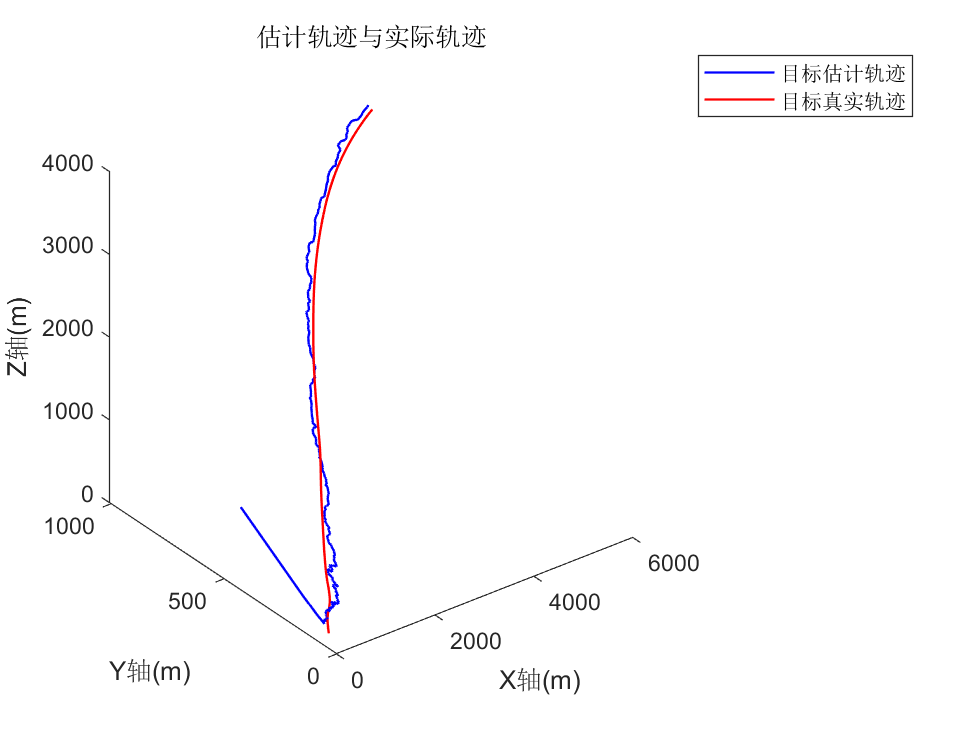
\includegraphics[width=0.8\textwidth]{Fig/预测运动轨迹与真实轨迹三维.png} %注意width=0.6\textwidth,个人认为这个比scale更为实用便捷
    \caption{三维预测运动轨迹与真实轨迹}
    \label{fig:预测运动轨迹与真实轨迹三维} %可加可不加,如果不用的话就不加,免得重复label而产生错误
\end{figure}

\begin{figure}  %插入一个图片最简单的方式
    \centering
    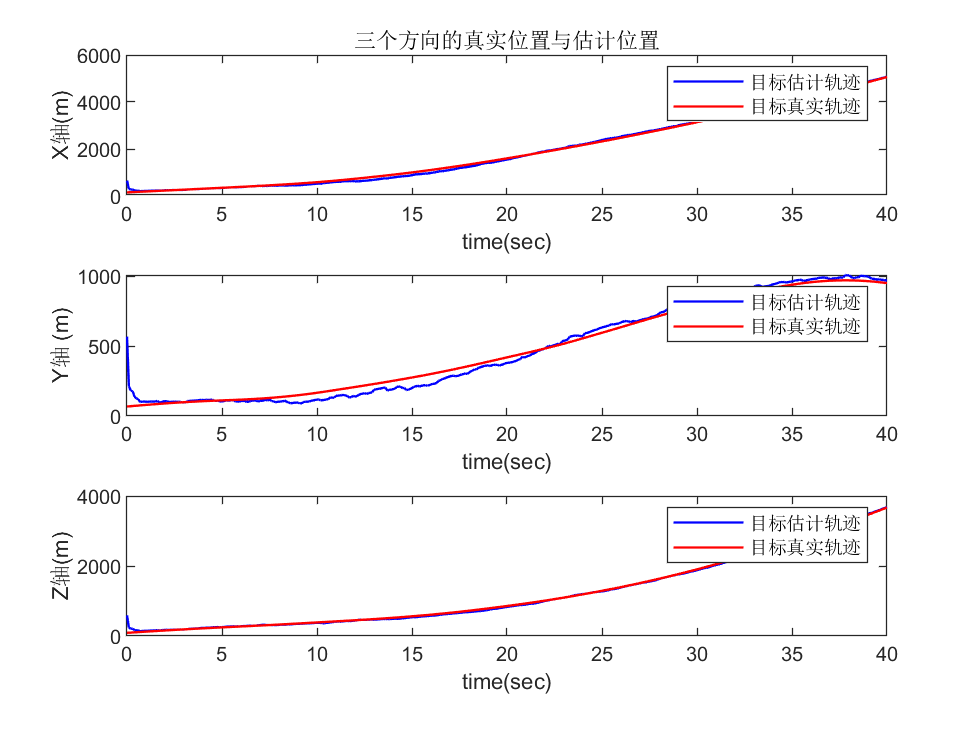
\includegraphics[width=0.8\textwidth]{Fig/三轴位置跟踪曲线.png} %注意width=0.6\textwidth,个人认为这个比scale更为实用便捷
    \caption{三轴位置跟踪曲线}
    \label{fig:三轴位置跟踪曲线} %可加可不加,如果不用的话就不加,免得重复label而产生错误
\end{figure}

\begin{figure}  %插入一个图片最简单的方式
    \centering
    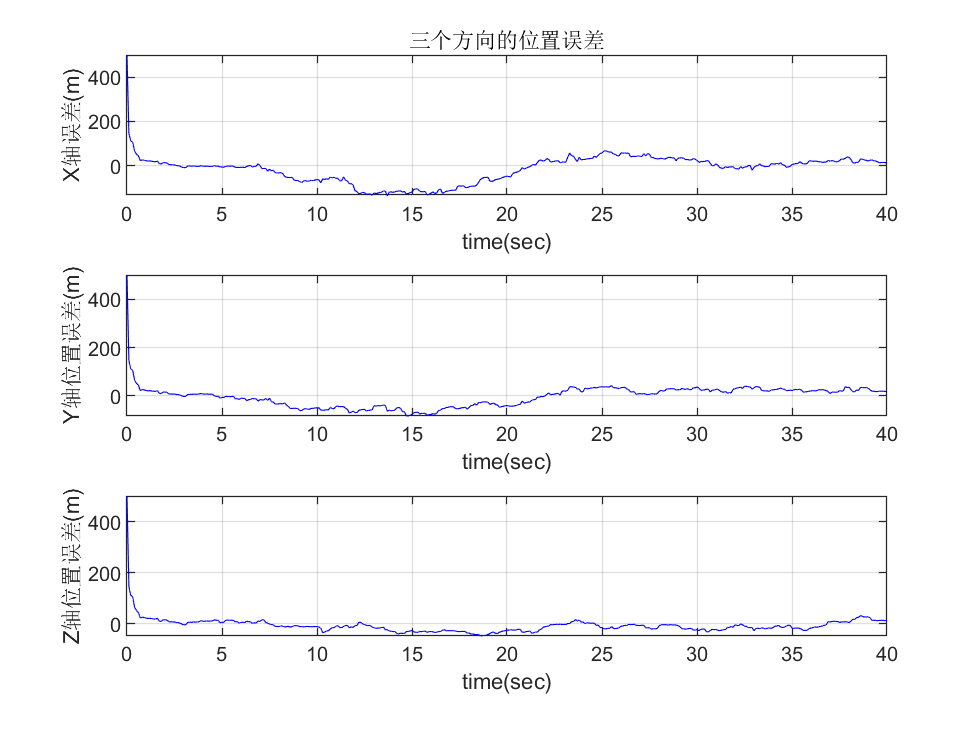
\includegraphics[width=0.8\textwidth]{Fig/位置误差曲线.png} %注意width=0.6\textwidth,个人认为这个比scale更为实用便捷
    \caption{位置误差曲线}
    \label{fig:位置误差曲线} %可加可不加,如果不用的话就不加,免得重复label而产生错误
\end{figure}

\begin{figure}  %插入一个图片最简单的方式
    \centering
    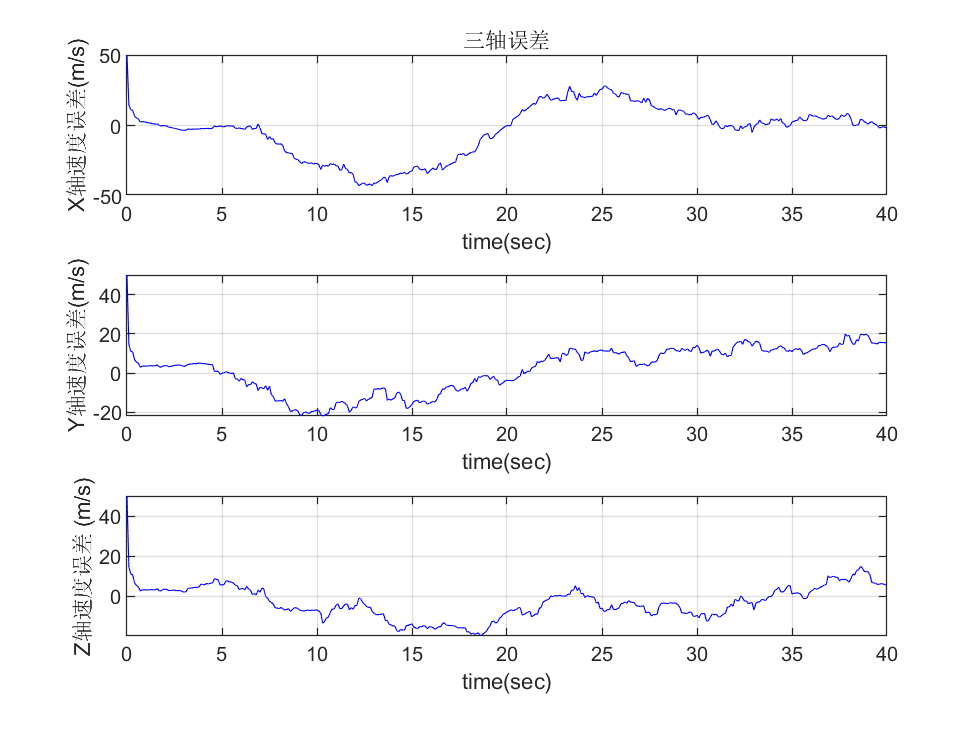
\includegraphics[width=0.8\textwidth]{Fig/速度误差曲线.png} %注意width=0.6\textwidth,个人认为这个比scale更为实用便捷
    \caption{速度误差曲线}
    %\label{fig:my_label} %可加可不加,如果不用的话就不加,免得重复label而产生错误
\end{figure}

\begin{figure}  %插入一个图片最简单的方式
    \centering
    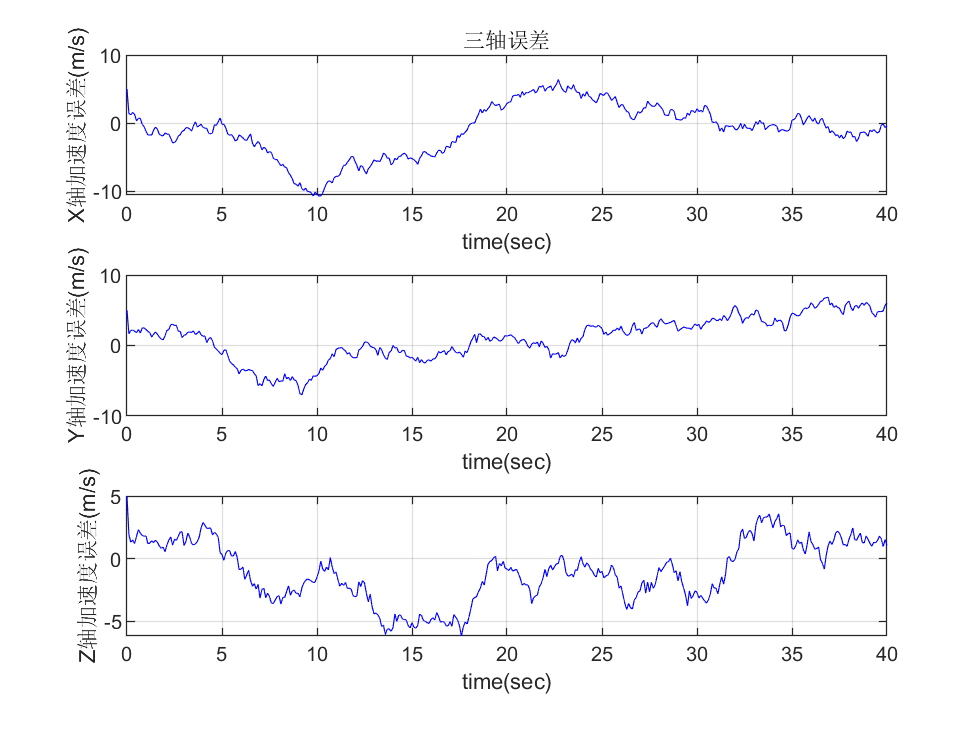
\includegraphics[width=0.8\textwidth]{Fig/加速度误差曲线.png} %注意width=0.6\textwidth,个人认为这个比scale更为实用便捷
    \caption{加速度误差曲线}
    \label{fig:加速度误差曲线} %可加可不加,如果不用的话就不加,免得重复label而产生错误
\end{figure}

\newpage

% \appendix
% \appendixname
\section{附录}
\lstinputlisting[language=Matlab]{EKF.m}

\end{document}